\documentclass[11pt]{article}

% ================= PACKAGES =================
\usepackage[a4paper,margin=0.95in]{geometry}
\usepackage{amsmath,amssymb,mathtools}
\usepackage{xcolor}
\usepackage{titlesec}
\usepackage{enumitem}
\usepackage{booktabs}
\usepackage[protrusion=true,expansion=false]{microtype}
\usepackage{fancyhdr}
\usepackage[most]{tcolorbox}
\usepackage{listings}
\usepackage{tikz}
\usetikzlibrary{positioning,arrows.meta,shapes.geometric,calc,fit,backgrounds,patterns}
\usepackage{pgfplots}
\pgfplotsset{compat=1.18}
\usepackage[hidelinks]{hyperref}

% ================= COLOURS =================
\definecolor{ink}{HTML}{0B2559}
\definecolor{accent}{HTML}{1D4ED8}
\definecolor{accent2}{HTML}{B45309}
\definecolor{green2}{HTML}{15803D}
\definecolor{codebg}{HTML}{F4F7FD}
\definecolor{codekw}{HTML}{1D4ED8}
\definecolor{codestr}{HTML}{15803D}
\definecolor{codecom}{HTML}{7A7A8C}
\definecolor{soft}{HTML}{4A5568}
\definecolor{defbg}{HTML}{E8EFFC}
\definecolor{actbg}{HTML}{FBF1E4}
\definecolor{dodbg}{HTML}{E8F5EC}

% ================= SECTION STYLE =================
\titleformat{\section}{\Large\bfseries\color{accent}}{\thesection}{0.7em}{}
\titleformat{\subsection}{\large\bfseries\color{ink}}{\thesubsection}{0.6em}{}
\titleformat{\subsubsection}{\normalsize\bfseries\color{accent2}}{\thesubsubsection}{0.5em}{}
\titlespacing*{\section}{0pt}{1.5em}{0.7em}
\titleformat{\part}{\Large\bfseries\color{accent}}{Part \thepart\ ~—~}{0pt}{}
\titlespacing*{\part}{0pt}{1.3em}{0.6em}

% ================= HEADER/FOOTER =================
\pagestyle{fancy}\fancyhf{}
\lhead{\small\color{soft}Trinetra-AI · PRD \& Build Guide}
\rhead{\small\color{soft}Implementation}
\cfoot{\small\color{soft}\thepage}
\renewcommand{\headrulewidth}{0.3pt}

% ================= CODE STYLE =================
\lstdefinestyle{code}{
  basicstyle=\ttfamily\footnotesize,
  keywordstyle=\color{codekw}\bfseries, stringstyle=\color{codestr},
  commentstyle=\color{codecom}\itshape, backgroundcolor=\color{codebg},
  frame=single, rulecolor=\color{codebg!60!gray}, framesep=5pt,
  breaklines=true, showstringspaces=false, columns=fullflexible,
  numbers=none, xleftmargin=6pt, xrightmargin=4pt, aboveskip=8pt, belowskip=6pt,
  literate={~}{{$\sim$}}1
}
\lstset{style=code}

% ================= CALLOUT BOXES =================
\newtcolorbox{defbox}[1][]{enhanced,breakable,colback=defbg,colframe=accent,
  boxrule=0pt,leftrule=3pt,arc=2pt,left=9pt,right=9pt,top=6pt,bottom=6pt,
  fonttitle=\bfseries,coltitle=accent,title={Requirement / Note#1}}
\newtcolorbox{actbox}[1][]{enhanced,breakable,colback=actbg,colframe=accent2,
  boxrule=0pt,leftrule=3pt,arc=2pt,left=9pt,right=9pt,top=6pt,bottom=6pt,
  fonttitle=\bfseries,coltitle=accent2,title={Action#1}}
\newtcolorbox{dodbox}{enhanced,breakable,colback=dodbg,colframe=green2,
  boxrule=0pt,leftrule=3pt,arc=2pt,left=9pt,right=9pt,top=6pt,bottom=6pt,
  fonttitle=\bfseries,coltitle=green2,title={Definition of Done}}

% ================= MATH SHORTCUTS =================
\newcommand{\vv}[1]{\mathbf{#1}}

\setlength{\parindent}{0pt}\setlength{\parskip}{5pt}

% ================================================================
\begin{document}

% ---------------- TITLE PAGE ----------------
\begin{titlepage}
\centering
\vspace*{1.8cm}
{\Huge\bfseries\color{accent} Trinetra-AI}\\[8pt]
{\LARGE\color{ink} Product Requirements \& Implementation Guide}\\[22pt]
{\large\color{soft}\textsc{From Dataset Download to Deployed System}}\\[8pt]
\rule{11.5cm}{0.5pt}\\[8pt]
{\normalsize\color{soft} An Intelligent Multi-Sensor Fusion Framework for GPS-Denied Navigation}\\[24pt]

\begin{tcolorbox}[width=12.9cm,colback=defbg,colframe=accent,boxrule=0pt,leftrule=3pt,arc=2pt]
\small
This document is the \textbf{execution plan} that turns the study phases (4--13) into a working
system. \textbf{Part~A} is a Product Requirements Document: what Trinetra-AI is, who it is for,
what it must do, and how success is measured. \textbf{Part~B} is a \textbf{step-by-step build
guide} --- environment setup, dataset download, preparation, EDA, preprocessing, features,
baseline fusion, AI modules, navigation, ROS~2 integration, evaluation, visualization, and
deployment --- each step with concrete actions, a \emph{Definition of Done}, and the pitfalls to
avoid. \textbf{Part~C} collects checklists. Follow it top to bottom.
\end{tcolorbox}
\vfill
{\small\color{soft} Requirements $\rightarrow$ data $\rightarrow$ baseline $\rightarrow$ intelligence $\rightarrow$ integration $\rightarrow$ evaluation $\rightarrow$ deployment.}

\vspace{6pt}
{\footnotesize\color{soft}\itshape Diagrams are native (TikZ) figures. Commands target Ubuntu~22.04 + ROS~2 Humble; adapt paths/versions to your setup. Verify every dataset licence on its official page before use.}
\end{titlepage}

\tableofcontents
\thispagestyle{fancy}
\newpage

% ================================================================
\part{Product Requirements Document}

\section{Product Overview}\label{sec:overview}

\subsection{Vision \& problem statement}

\begin{defbox}
\textbf{Vision.} Trinetra-AI is a modular, AI-enhanced multi-sensor fusion framework that
estimates a platform's position, velocity, and orientation \emph{accurately and continuously
when GPS is unavailable, degraded, or denied} --- indoors, in urban canyons, underground, or
under jamming.

\textbf{Problem.} Inertial-only navigation drifts without bound; GPS fails in exactly the
environments where navigation matters most. Trinetra-AI closes this gap by fusing inertial,
magnetic, barometric, and (future) quantum-magnetometer / visual / LiDAR sensing with learned
error models and absolute magnetic map-matching.
\end{defbox}

\subsection{Goals and non-goals}

\begin{center}\footnotesize
\begin{tabular}{@{}p{6.2cm}p{6.2cm}@{}}
\toprule
\textbf{Goals (in scope)} & \textbf{Non-goals (out of scope, for now)}\\
\midrule
Drift-bounded GPS-denied state estimation & Building physical quantum hardware\\
AI modules that de-noise sensors \& adapt the filter & Full autonomous path planning / mission autonomy\\
Absolute anchoring via magnetic map-matching & Multi-robot swarms\\
A reproducible, ROS~2-deployable software system & Certified safety-critical avionics\\
Rigorous evaluation on public + simulated data & A commercial product\\
\bottomrule
\end{tabular}
\end{center}

\subsection{The one-sentence definition of success}

\begin{dodbox}
Trinetra-AI succeeds if, on a held-out GPS-denied trajectory, it produces a
\textbf{position estimate whose error grows substantially slower than a classical inertial
baseline}, runs in \textbf{real time on an edge device}, and every reported number is
\textbf{reproducible} from versioned code + data + config.
\end{dodbox}

% ================================================================
\section{Users \& Use Cases}\label{sec:users}

\begin{center}\footnotesize
\begin{tabular}{@{}p{3.0cm}p{4.6cm}p{4.6cm}@{}}
\toprule
\textbf{User} & \textbf{Needs} & \textbf{Primary use case}\\
\midrule
You (developer/researcher) & reproducible experiments, clear metrics & build, train, evaluate, iterate\\
A robot / vehicle & real-time pose under GPS denial & on-board live navigation\\
A reviewer / collaborator & to reproduce your results & clone repo, run one command, get the number\\
Future extension & swap in quantum/LiDAR/camera & plug a new sensor behind the interface\\
\bottomrule
\end{tabular}
\end{center}

\textbf{Representative scenarios.} (1) A ground vehicle drives through a tunnel: GPS drops, the
filter enters denied mode, magnetic map-matching + inertial keep the error bounded until GPS
returns. (2) A pedestrian/handheld unit navigates indoors from IMU + magnetometer alone.
(3) A drone loses GPS under jamming and holds position using inertial + barometric + magnetic
fusion.

% ================================================================
\section{Scope, Assumptions \& Dependencies}\label{sec:scope}

\begin{defbox}
\textbf{Assumptions.} (1) Development on Ubuntu~22.04 with ROS~2 Humble; deployment target is an
NVIDIA Jetson. (2) Initial sensors are those with public data --- IMU (accel+gyro),
magnetometer, GPS (for ground truth / denial simulation), barometer. (3) Quantum magnetometer,
LiDAR, camera, wheel encoder, atomic clock are \emph{future} channels behind the same
interfaces. (4) Evaluation uses public datasets first (no hardware required to start), then
simulation, then optional real hardware.
\end{defbox}

\begin{center}\footnotesize
\begin{tabular}{@{}p{3.4cm}p{9.0cm}@{}}
\toprule
\textbf{Dependency} & \textbf{Role}\\
\midrule
Python 3.10+, NumPy/SciPy/pandas & core scientific stack\\
PyTorch & AI modules (Phase 9)\\
ROS~2 Humble + robot\_localization & middleware + fusion node (Phase 10)\\
TimescaleDB / Parquet / DVC / MLflow & data \& experiment management (Phases 11, 13)\\
Gazebo (Fortress/Harmonic) & simulation \& GPS-denial testing\\
Docker & reproducible environment \& deployment\\
Public datasets & RoNIN, TLIO, OxIOD, EuRoC, KITTI, comma2k19, MagNav (Sec \ref{sec:data})\\
\bottomrule
\end{tabular}
\end{center}

% ================================================================
\section{Functional Requirements}\label{sec:fr}

\begin{center}\footnotesize
\begin{tabular}{@{}p{1.3cm}p{7.4cm}p{3.6cm}@{}}
\toprule
\textbf{ID} & \textbf{Requirement} & \textbf{Phase}\\
\midrule
FR-1 & Ingest multi-rate sensor streams (IMU 100--200\,Hz, mag, GPS 1\,Hz, baro) from datasets, bags, or live drivers & 6, 11\\
FR-2 & Time-synchronise \& resample all streams to a common grid; mask gaps & 4, 11\\
FR-3 & Calibrate sensors (bias, scale, hard/soft-iron for magnetometer) & 6\\
FR-4 & Compute windowed features (statistical, spectral, lags) & 4, 11\\
FR-5 & Fuse sensors via EKF/UKF into a pose+velocity+bias state & 7\\
FR-6 & De-noise raw inertial signals with a learned model & 9\\
FR-7 & Predict \& correct inertial drift / bias with AI & 9\\
FR-8 & Detect sensor faults / anomalies and score confidence & 9\\
FR-9 & Adapt filter noise ($\vv{Q},\vv{R}$) from confidence/anomaly signals & 7, 9\\
FR-10 & Provide absolute correction via magnetic map-matching (GPS-denied) & 8\\
FR-11 & Simulate GPS denial (mask GPS) and enter/exit denied mode cleanly & 8\\
FR-12 & Expose everything as ROS~2 nodes/topics with a correct TF tree & 10\\
FR-13 & Record/replay sessions (MCAP) for deterministic testing & 10, 11\\
FR-14 & Visualise trajectory, error, sensor health (RViz2 + dashboards) & 12\\
FR-15 & Track experiments (code+data+metrics) reproducibly & 13\\
\bottomrule
\end{tabular}
\end{center}

% ================================================================
\section{Non-Functional Requirements}\label{sec:nfr}

\begin{center}\footnotesize
\begin{tabular}{@{}p{1.3cm}p{4.0cm}p{7.0cm}@{}}
\toprule
\textbf{ID} & \textbf{Attribute} & \textbf{Target}\\
\midrule
NFR-1 & Accuracy & GPS-denied position error grows markedly slower than a strapdown-INS / naive double-integration baseline (quantified in Sec \ref{sec:metrics})\\
NFR-2 & Real-time & on-vehicle loop keeps up with sensor rate (e.g.\ 200\,Hz $\Rightarrow$ $<$5\,ms/sample budget) on the Jetson\\
NFR-3 & Reproducibility & any result re-derivable from a commit SHA + data version + config\\
NFR-4 & Modularity & add/swap a sensor or AI module without editing the core\\
NFR-5 & Portability & identical run via Docker on laptop and Jetson\\
NFR-6 & Reliability & graceful degradation when a sensor drops; no NaNs/crashes\\
NFR-7 & Observability & live health/anomaly signals + logs for every run\\
\bottomrule
\end{tabular}
\end{center}

% ================================================================
\section{System Architecture (recap)}\label{sec:arch}

The build realises the clean, layered architecture from Phase~13: a pure algorithmic core,
ROS~2 adapters, sensor/AI plugins, and a data pipeline feeding both training and the live loop.

\begin{center}
\resizebox{\textwidth}{!}{%
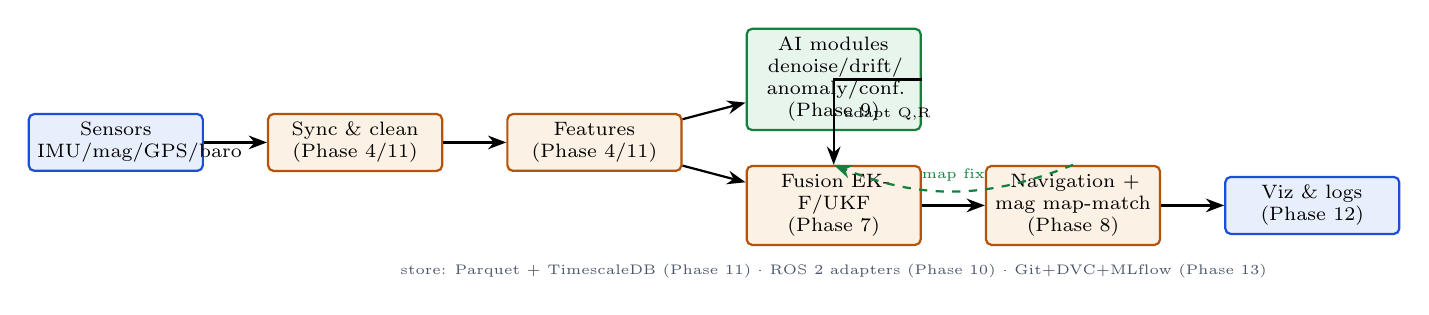
\begin{tikzpicture}[font=\scriptsize,>={Stealth[]},node distance=3.4mm and 8mm,
  s/.style={draw=accent,rounded corners=2pt,fill=defbg,inner sep=3pt,align=center,text width=2.0cm},
  p/.style={draw=accent2,rounded corners=2pt,fill=actbg,inner sep=3pt,align=center,text width=2.0cm},
  a/.style={draw=green2,rounded corners=2pt,fill=dodbg,inner sep=3pt,align=center,text width=2.0cm},thick]
\node[s](sens){Sensors\\IMU/mag/GPS/baro};
\node[p,right=of sens](sync){Sync \& clean\\(Phase 4/11)};
\node[p,right=of sync](feat){Features\\(Phase 4/11)};
\node[a,right=of feat,yshift=8mm](ai){AI modules\\denoise/drift/\\anomaly/conf.\\(Phase 9)};
\node[p,right=of feat,yshift=-8mm](fus){Fusion EKF/UKF\\(Phase 7)};
\node[p,right=of fus](nav){Navigation +\\mag map-match\\(Phase 8)};
\node[s,right=of nav](viz){Viz \& logs\\(Phase 12)};
\draw[->](sens)--(sync);\draw[->](sync)--(feat);
\draw[->](feat)--(ai);\draw[->](feat)--(fus);
\draw[->](ai.east)-|(fus.north) node[pos=0.7,right,font=\tiny]{adapt Q,R};
\draw[->](fus)--(nav);\draw[->](nav)--(viz);
\draw[->,green2,dashed](nav.north) to[bend left=22] node[above,font=\tiny]{map fix} (fus.north);
\node[soft,below=1mm of fus,font=\tiny]{store: Parquet + TimescaleDB (Phase 11) · ROS 2 adapters (Phase 10) · Git+DVC+MLflow (Phase 13)};
\end{tikzpicture}%
}
\end{center}

\begin{defbox}
The \textbf{two data regimes} run on the same code: an \emph{offline} pipeline (download $\to$
prepare $\to$ train $\to$ evaluate) and an \emph{online} pipeline (live sensors $\to$ sync $\to$
features $\to$ AI $\to$ fusion $\to$ navigation), with train/serve parity guaranteed by sharing
the feature and model code. Build the offline pipeline first (Steps 1--10), then wrap it in
ROS~2 for the online loop (Step 9) and deploy (Step 12).
\end{defbox}

% ================================================================
\section{Success Metrics \& Acceptance Criteria}\label{sec:metrics}

\begin{center}\footnotesize
\begin{tabular}{@{}p{3.4cm}p{4.6cm}p{4.4cm}@{}}
\toprule
\textbf{Metric} & \textbf{Definition} & \textbf{Acceptance target}\\
\midrule
ATE & RMSE of estimated vs ground-truth positions over a trajectory & beats the INS/naive baseline by a clear margin\\
RTE & relative trajectory error over fixed windows (e.g.\ 60\,s) & lower than baseline; stable across trajectories\\
Drift rate & position error growth per minute in GPS-denied mode & sub-linear vs unaided inertial\\
Attitude error & RMSE of roll/pitch/yaw & within a few degrees\\
Real-time factor & processing time / data time on Jetson & $\le 1.0$ (keeps up)\\
Reproducibility & re-run $\Rightarrow$ identical metrics & bit-for-bit on fixed seed/data\\
Calibration (AI conf.) & predicted confidence vs actual error & well-calibrated (reliability diagram)\\
\bottomrule
\end{tabular}
\end{center}

\begin{dodbox}
The project is \emph{accepted} when, on at least two held-out GPS-denied trajectories: (i)
Trinetra-AI's ATE and drift rate beat a documented inertial baseline; (ii) the full stack runs
in real time in simulation (and ideally on a Jetson); (iii) every headline number is
reproduced by a single scripted command from versioned code+data. Record all three in the
README.
\end{dodbox}

% ================================================================
\section{Milestones \& Timeline}\label{sec:milestones}

\begin{center}
\resizebox{\textwidth}{!}{%
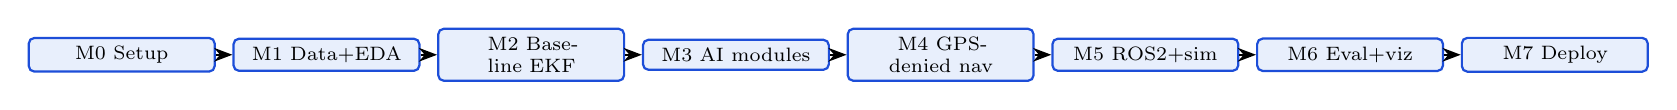
\begin{tikzpicture}[font=\scriptsize,>={Stealth[]},
  ms/.style={draw=accent,fill=defbg,rounded corners=2pt,inner sep=3pt,align=center,text width=2.15cm},thick]
\foreach \i/\name/\x in {0/{M0 Setup}/0, 1/{M1 Data+EDA}/2.6, 2/{M2 Baseline EKF}/5.2,
  3/{M3 AI modules}/7.8, 4/{M4 GPS-denied nav}/10.4, 5/{M5 ROS2+sim}/13.0,
  6/{M6 Eval+viz}/15.6, 7/{M7 Deploy}/18.2}
  \node[ms] (m\i) at (\x,0) {\name};
\foreach \a/\b in {0/1,1/2,2/3,3/4,4/5,5/6,6/7} \draw[->](m\a)--(m\b);
\end{tikzpicture}%
}
\end{center}

\begin{center}\footnotesize
\begin{tabular}{@{}p{1.1cm}p{4.6cm}p{6.4cm}@{}}
\toprule
\textbf{M} & \textbf{Milestone} & \textbf{Deliverable / exit criterion}\\
\midrule
M0 & Environment \& repo & repo scaffolded; Docker builds; CI green; DVC/MLflow wired\\
M1 & Data + EDA & $\ge$1 dataset in canonical schema; EDA report; quality checks pass\\
M2 & Baseline fusion & EKF/UKF runs end-to-end; baseline ATE/RTE recorded\\
M3 & AI modules & denoise+drift+anomaly+confidence trained; each beats no-AI ablation\\
M4 & GPS-denied navigation & magnetic map-match + denied-mode; error bounded vs unaided INS\\
M5 & ROS~2 + simulation & full node graph runs in Gazebo; GPS-denial simulated\\
M6 & Evaluation + visualization & benchmark table + ablations; trajectory/health dashboards\\
M7 & Deployment & Dockerised stack on Jetson (or documented sim deployment)\\
\bottomrule
\end{tabular}
\end{center}

\begin{defbox}
Treat each milestone as a \textbf{vertical slice} that ends in working, tested, tagged software
--- not a horizontal layer. Ship M2 (a working baseline on real data) before polishing any single
AI module; a mediocre end-to-end system beats a perfect component that connects to nothing.
\end{defbox}

% ================================================================
\section{Risks \& Mitigations}\label{sec:risks}

\begin{center}\footnotesize
\begin{tabular}{@{}p{4.4cm}p{8.0cm}@{}}
\toprule
\textbf{Risk} & \textbf{Mitigation}\\
\midrule
No magnetic-anomaly ground data on hand & start with inertial datasets (RoNIN/TLIO); add MagNav data for the magnetic path; simulate magnetic field in Gazebo\\
AI modules overfit / don't beat baseline & always compare against an ablation; keep the classical baseline as fallback; use held-out subjects/trajectories\\
Timing/sync bugs read as ``sensor error'' & rigorous Step~4 sync; unit-test alignment; never interpolate across long gaps\\
Scope creep (planning, SLAM, quantum HW) & keep them out of the core; interfaces-only for future sensors\\
Real-time budget blown on Jetson & profile early; export to ONNX/TensorRT; compose nodes; drop to lighter models\\
Irreproducible results & Git+DVC+MLflow from M0; seed control; Docker; tag every result\\
Dataset licence constraints & verify each licence; use only permitted (non-commercial/research) data; document provenance\\
\bottomrule
\end{tabular}
\end{center}

% ================================================================
\part{Step-by-Step Implementation Guide}

The build proceeds as a linear pipeline. Each step lists its \emph{objective}, \emph{actions}
(commands/code), \emph{outputs}, a \emph{Definition of Done}, and \emph{pitfalls}.

\begin{center}
\resizebox{\textwidth}{!}{%
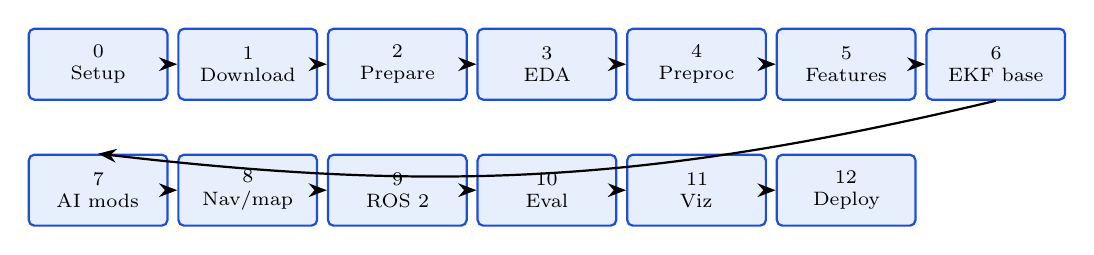
\begin{tikzpicture}[font=\scriptsize,>={Stealth[]},node distance=2.4mm and 4.2mm,
  b/.style={draw=accent,rounded corners=2pt,fill=defbg,inner sep=3pt,align=center,text width=1.55cm,minimum height=0.9cm},thick]
\foreach \i/\t/\x in {0/{0\\Setup}/0, 1/{1\\Download}/1.9, 2/{2\\Prepare}/3.8, 3/{3\\EDA}/5.7,
  4/{4\\Preproc}/7.6, 5/{5\\Features}/9.5, 6/{6\\EKF base}/11.4}
  \node[b] (a\i) at (\x,0) {\t};
\foreach \i/\t/\x in {7/{7\\AI mods}/0, 8/{8\\Nav/map}/1.9, 9/{9\\ROS 2}/3.8,
  10/{10\\Eval}/5.7, 11/{11\\Viz}/7.6, 12/{12\\Deploy}/9.5}
  \node[b] (c\i) at (\x,-1.6) {\t};
\foreach \a/\b in {0/1,1/2,2/3,3/4,4/5,5/6} \draw[->](a\a)--(a\b);
\foreach \a/\b in {7/8,8/9,9/10,10/11,11/12} \draw[->](c\a)--(c\b);
\draw[->](a6.south) to[bend left=10] (c7.north);
\end{tikzpicture}%
}
\end{center}

% ---------------- STEP 0 ----------------
\section{Step 0 --- Environment \& Repository Setup}\label{sec:step0}

\textbf{Objective.} A reproducible development environment and a scaffolded repository with
version control, data versioning, and CI in place \emph{before} any data is touched.

\begin{actbox}
\begin{lstlisting}[language=bash]
# 1. System + ROS 2 Humble (Ubuntu 22.04). Then a Python env:
python3 -m venv .venv && source .venv/bin/activate
pip install numpy scipy pandas matplotlib scikit-learn h5py pyarrow \
            torch mlflow dvc great_expectations jupyter ruff black pytest

# 2. Scaffold the repo (mirrors Phase 13 structure)
mkdir -p trinetra-ai/{src/trinetra_core/{sensor_fusion,navigation,ai_modules,pipelines},\
src/ros2,configs,datasets,models,visualization,tests,docs,research,docker,scripts,\
.github/workflows}
cd trinetra-ai && git init && git branch -M main

# 3. Data + experiment versioning
dvc init
dvc remote add -d store <your-remote-url>     # S3/GDrive/local
mlflow ui &                                    # experiment dashboard at :5000

# 4. First commit + tag
printf "trinetra_core/**/__pycache__\n.venv/\ndatasets/**/*.parquet\n" > .gitignore
git add . && git commit -m "chore: scaffold repo (M0)"
git tag -a v0.0-setup -m "environment ready"
\end{lstlisting}
\end{actbox}

\begin{defbox}
Create \texttt{pyproject.toml} (pin dependency versions), a \texttt{Dockerfile}
(\texttt{FROM ros:humble}, install the same deps), and a minimal CI workflow
(\texttt{.github/workflows/ci.yaml}) that runs \texttt{ruff} + \texttt{pytest}. Everything you
add from here flows through Git (code), DVC (data/models), and MLflow (runs).
\end{defbox}

\begin{dodbox}
\texttt{python -c "import torch, pandas"} works; \texttt{ros2 --help} works; \texttt{git log}
shows the tagged scaffold commit; \texttt{dvc status} and \texttt{mlflow ui} run; the Docker
image builds. You can now reproduce the environment on any machine.
\end{dodbox}

% ---------------- STEP 1 ----------------
\section{Step 1 --- Dataset Selection \& Download}\label{sec:data}

\textbf{Objective.} Obtain real multi-sensor navigation data so you can build and evaluate
\emph{without hardware}. Start with inertial datasets; add magnetic \& driving data for the
GPS-denied and fusion paths.

\begin{center}\footnotesize
\begin{tabular}{@{}p{2.2cm}p{3.4cm}p{2.0cm}p{4.0cm}@{}}
\toprule
\textbf{Dataset} & \textbf{Sensors / truth} & \textbf{Best for} & \textbf{Source (verify licence)}\\
\midrule
\textbf{RoNIN} & IMU+mag, 3D truth, 200\,Hz & inertial AI, start here & ronin.cs.sfu.ca (FRDR; $\sim$50\% public, research licence)\\
TLIO & IMU, VIO truth & learned inertial + EKF & github.com/CathIAS/TLIO\\
OxIOD & IMU (accel/gyro/mag) & inertial baselines & official OxIOD page\\
EuRoC MAV & IMU+stereo, MoCap truth & VIO / fusion & projects.asl.ethz.ch (ETH ASL)\\
KITTI & IMU+GPS+LiDAR+cam, RTK truth & driving-scale fusion & cvlibs.net/datasets/kitti\\
comma2k19 & IMU+GNSS+CAN & GPS/INS driving & github.com/commaai/comma2k19\\
MagNav (DAF-MIT) & aeromagnetic + INS & magnetic map-match & github.com/MIT-AI-Accelerator/MagNav.jl\\
\bottomrule
\end{tabular}
\end{center}

\begin{actbox}
\begin{lstlisting}[language=bash]
# Recommended starting point: RoNIN (agree to the research licence on the site first)
#   Download the public split from ronin.cs.sfu.ca (FRDR repository), then:
mkdir -p datasets/raw/ronin && cd datasets/raw/ronin
#   ... place the downloaded .hdf5 sequences here ...

# TLIO (code + data pointers):
git clone https://github.com/CathIAS/TLIO third_party/TLIO

# EuRoC (one sequence, ASL format / rosbag):
mkdir -p datasets/raw/euroc && cd datasets/raw/euroc
#   download e.g. "Machine Hall 01" from the ETH ASL page

# Track raw data with DVC (pointers in Git, blobs in your remote)
cd $REPO && dvc add datasets/raw/ronin && git add datasets/raw/ronin.dvc .gitignore
git commit -m "data: add RoNIN raw (v1)" && dvc push
\end{lstlisting}
\end{actbox}

\begin{defbox}
\textbf{Why RoNIN first:} it is large (42.7\,h), 200\,Hz, has accel+gyro+\emph{magnetometer}
and 3-D ground truth, and directly matches the inertial-AI core. Use \textbf{EuRoC/KITTI} when
you add the visual/GPS fusion paths and \textbf{MagNav} for the magnetic-anomaly path. Always
keep an immutable \texttt{datasets/raw/} and never edit it in place.
\end{defbox}

\begin{dodbox}
At least one dataset is downloaded into \texttt{datasets/raw/}, DVC-tracked and pushed to your
remote, with its licence noted in \texttt{datasets/README.md}. \texttt{dvc pull} on a fresh
clone restores it.
\end{dodbox}

\textbf{Pitfalls.} Committing raw data to Git (use DVC); ignoring the licence (RoNIN is
research-only, $\sim$50\% public); assuming all datasets share units/axes/frames --- they do not
(Step~2 fixes this).

% ---------------- STEP 2 ----------------
\section{Step 2 --- Dataset Preparation (Canonical Schema)}\label{sec:prep}

\textbf{Objective.} Convert every dataset's idiosyncratic format into \emph{one canonical
schema} (consistent columns, units, frames, timestamps) so all downstream code is
dataset-agnostic.

\begin{defbox}
\textbf{Canonical row:} \texttt{t} (seconds, monotonic), \texttt{ax,ay,az} (m/s\textsuperscript{2}),
\texttt{gx,gy,gz} (rad/s), \texttt{mx,my,mz} ($\mu$T), optional \texttt{lat,lon,alt} / local
\texttt{x,y,z} truth, \texttt{baro} (Pa). One \textbf{adapter per dataset} maps into this; the
rest of the system only ever sees the canonical form. Store as \textbf{Parquet} (+Zstd).
\end{defbox}

\begin{actbox}
\begin{lstlisting}[language=Python]
# src/trinetra_core/pipelines/adapters.py -- one function per dataset
import pandas as pd, numpy as np, h5py

CANON = ["t","ax","ay","az","gx","gy","gz","mx","my","mz","gt_x","gt_y","gt_z"]

def load_ronin(path):
    with h5py.File(path, "r") as f:
        acc  = f["synced/acce"][:]      # (N,3) m/s^2
        gyro = f["synced/gyro"][:]      # (N,3) rad/s
        mag  = f["synced/magnet"][:]    # (N,3) uT
        t    = f["synced/time"][:]      # seconds
        gt   = f["pose/tango_pos"][:]   # (N,3) ground-truth position
    df = pd.DataFrame({"t": t,
        "ax":acc[:,0],"ay":acc[:,1],"az":acc[:,2],
        "gx":gyro[:,0],"gy":gyro[:,1],"gz":gyro[:,2],
        "mx":mag[:,0],"my":mag[:,1],"mz":mag[:,2],
        "gt_x":gt[:,0],"gt_y":gt[:,1],"gt_z":gt[:,2]})
    return df[CANON]

def to_canonical(df, out):
    df.to_parquet(out, compression="zstd")   # one interface for everything downstream
\end{lstlisting}
\end{actbox}

\begin{dodbox}
Running the adapter on a raw sequence yields a canonical Parquet file with correct units and a
monotonic timestamp. A second dataset's adapter produces the \emph{same} columns. Downstream
code imports neither HDF5 nor dataset names.
\end{dodbox}

\textbf{Pitfalls.} Unit mix-ups (g vs m/s\textsuperscript{2}; deg/s vs rad/s); axis/frame
conventions differ per dataset (check each spec); non-monotonic or duplicated timestamps.

% ---------------- STEP 3 ----------------
\section{Step 3 --- Exploratory Data Analysis (EDA)}\label{sec:eda}

\textbf{Objective.} \emph{Understand and sanity-check} the data before modelling: rates,
ranges, noise, gaps, drift, and cross-sensor consistency. EDA prevents weeks of debugging a
``model'' problem that is really a data problem.

\begin{actbox}
\begin{lstlisting}[language=Python]
# notebooks/03_eda.ipynb -- the essential checks
import pandas as pd, numpy as np, matplotlib.pyplot as plt
df = pd.read_parquet("datasets/interim/ronin_seq01.parquet")

# (a) sampling rate & gaps
dt = np.diff(df["t"]); fs = 1/np.median(dt)
print("median rate:", round(fs,1), "Hz | max gap:", round(dt.max()*1000,1), "ms")

# (b) ranges / physical plausibility
print(df[["ax","ay","az"]].describe())          # |a| ~ 9.8 at rest?
print("gyro max |w| (rad/s):", np.abs(df[["gx","gy","gz"]]).max().max())

# (c) time-series & spectra (look for drift, spikes, bias)
fig,ax = plt.subplots(3,1,figsize=(9,6))
ax[0].plot(df["t"], df[["ax","ay","az"]]); ax[0].set_title("accel")
ax[1].plot(df["t"], df[["gx","gy","gz"]]); ax[1].set_title("gyro")
ax[2].magnitude_spectrum(df["az"]-df["az"].mean(), Fs=fs); ax[2].set_title("accel-z spectrum")

# (d) ground-truth trajectory & path length
gt = df[["gt_x","gt_y"]].values
print("path length (m):", np.linalg.norm(np.diff(gt,axis=0),axis=1).sum())
plt.figure(); plt.plot(gt[:,0], gt[:,1]); plt.axis("equal"); plt.title("GT trajectory")

# (e) Allan variance (noise characterisation -> Q/R priors, Phase 6)
#     use allantools on a static segment to get ARW / bias instability
\end{lstlisting}
\end{actbox}

\begin{defbox}
\textbf{What EDA must answer:} Is the sampling rate what the docs claim? Are there gaps/dropouts?
Are magnitudes physical (gravity $\approx 9.8$ at rest)? Is there visible bias/drift? What do the
spectra say about noise bands (informs Phase~5 filtering)? What does the ground-truth trajectory
look like? Allan variance on a static segment gives the noise coefficients that seed the Kalman
filter's $\vv{Q},\vv{R}$ (Phase~6/7).
\end{defbox}

\begin{dodbox}
An EDA notebook/report exists per dataset covering rate, gaps, ranges, spectra, trajectory, and
noise (Allan). You can state each sensor's effective rate, noise level, and any anomalies in one
paragraph --- and you have Q/R priors for Step~6.
\end{dodbox}

\textbf{Pitfalls.} Skipping EDA and trusting the docs; missing a silent rate mismatch or a long
GPS gap; not checking gravity magnitude (catches unit/axis errors instantly).

% ---------------- STEP 4 ----------------
\section{Step 4 --- Preprocessing, Sync \& Calibration}\label{sec:preproc}

\textbf{Objective.} Turn raw canonical data into clean, aligned, calibrated signals on a common
time grid --- the single most bug-prone and most important transformation in the whole system.

\begin{actbox}
\begin{lstlisting}[language=Python]
# src/trinetra_core/pipelines/preprocess.py
import numpy as np, pandas as pd

def align_to_grid(df, fs=200.0):
    t = df["t"].values; grid = np.arange(t[0], t[-1], 1.0/fs)
    out = {"t": grid}
    for c in df.columns.drop("t"):
        out[c] = np.interp(grid, t, df[c].values)   # do NOT interp across long gaps
    return pd.DataFrame(out)

def calibrate_mag(m, hard_iron, soft_iron):
    return (m - hard_iron) @ soft_iron.T             # Phase 6 hard/soft-iron

def remove_bias(x, static_mask):
    return x - x[static_mask].mean(0)                # gyro/accel bias from a still segment

def lowpass(x, fs, fc=25.0, order=4):                # Phase 5 anti-alias / de-noise
    from scipy.signal import butter, filtfilt
    b,a = butter(order, fc/(fs/2)); return filtfilt(b,a,x,axis=0)
\end{lstlisting}
\end{actbox}

\begin{defbox}
Order matters: (1) mask long gaps (do \emph{not} fabricate data across them --- flag denied mode
instead); (2) resample all channels to a common grid; (3) remove biases from a static segment;
(4) apply hard/soft-iron magnetometer calibration; (5) band-limit with a filter matched to the
noise spectra from EDA. Sub-millisecond misalignment at high dynamics shows up downstream as
``sensor error'' that is really \emph{timing} error.
\end{defbox}

\begin{dodbox}
A \texttt{preprocess} function turns a canonical Parquet into a synced, calibrated, gap-masked
Parquet on a fixed grid. Unit tests confirm alignment (known inputs $\to$ known grid) and that
gaps are masked, not interpolated. Gravity magnitude is $\approx 9.8$ post-calibration.
\end{dodbox}

\textbf{Pitfalls.} Interpolating across long dropouts (fabricates motion); calibrating on a
non-static segment; filtering away real signal with too-low a cutoff; forgetting that resampling
changes effective noise.

% ---------------- STEP 5 ----------------
\section{Step 5 --- Feature Engineering}\label{sec:features}

\textbf{Objective.} Turn the clean signal into the windowed features the AI modules consume ---
using \emph{one} feature function shared by training and the live loop (train/serve parity).

\begin{actbox}
\begin{lstlisting}[language=Python]
# src/trinetra_core/pipelines/features.py -- SAME code offline & online (no skew)
import numpy as np

def window_features(w, fs=200.0):
    """w: (L, C) window of synced channels -> feature dict."""
    fft = np.abs(np.fft.rfft(w, axis=0))
    freqs = np.fft.rfftfreq(w.shape[0], 1/fs)
    return {
        "mean": w.mean(0), "std": w.std(0),
        "rms":  np.sqrt((w**2).mean(0)),
        "energy": (w**2).sum(0),
        "dom_freq": freqs[fft.argmax(0)],
        "spec_low":  fft[freqs < 5].sum(0),
        "spec_high": fft[freqs >= 5].sum(0),
        "jerk_rms": np.sqrt((np.diff(w,axis=0)**2).mean(0)),
    }

def make_windows(df, L=200, stride=10):              # Phase 4 windowing
    X = df[["ax","ay","az","gx","gy","gz"]].values
    return np.stack([X[i:i+L] for i in range(0, len(X)-L, stride)])
\end{lstlisting}
\end{actbox}

\begin{dodbox}
A versioned \texttt{features} table (Parquet) exists, produced by a single function that the
online loop will also call. Windowing matches the model's expected input. Feature version is
recorded (e.g.\ in MLflow) so training and serving cannot silently diverge.
\end{dodbox}

\textbf{Pitfalls.} Different feature code for train vs serve (the classic skew bug); leaking
future data into a window; unversioned features.

% ---------------- STEP 6 ----------------
\section{Step 6 --- Baseline Sensor Fusion (EKF/UKF)}\label{sec:ekf}

\textbf{Objective.} A working \emph{classical} fusion baseline end-to-end. This is the number
every AI improvement is measured against --- build it before any learning.

\begin{actbox}
\begin{lstlisting}[language=Python]
# src/trinetra_core/sensor_fusion/ekf.py -- minimal error-state EKF skeleton (Phase 7)
import numpy as np

class EKF:
    def __init__(self, dim, Q, R):
        self.x = np.zeros(dim); self.P = np.eye(dim)
        self.Q = Q; self.R = R                          # Q/R seeded from Allan variance (Step 3)
    def predict(self, F, u=None):
        self.x = F @ self.x
        self.P = F @ self.P @ F.T + self.Q
    def update(self, z, H):
        y = z - H @ self.x                              # innovation
        S = H @ self.P @ H.T + self.R
        K = self.P @ H.T @ np.linalg.inv(S)             # Kalman gain
        self.x = self.x + K @ y
        self.P = (np.eye(len(self.x)) - K @ H) @ self.P
        return y                                        # expose innovation (feeds Phase 9 anomaly)
\end{lstlisting}
\end{actbox}

\begin{defbox}
Start with \texttt{robot\_localization}'s EKF (Phase 10) or the skeleton above; state = position,
velocity, orientation, biases. Predict with the IMU mechanization (Phase 8), update with GPS
(when present) / zero-velocity / magnetic heading. Run it over a full trajectory and compute ATE/
RTE vs ground truth --- that is your \textbf{baseline row}.
\end{defbox}

\begin{dodbox}
The EKF runs over a whole sequence without diverging, produces a trajectory, and you have logged
its ATE/RTE. A GPS-denied variant (mask GPS) shows the expected drift. These numbers are recorded
in MLflow as the baseline every later step must beat.
\end{dodbox}

\textbf{Pitfalls.} Wrong $\vv{Q}/\vv{R}$ scaling (filter diverges or ignores measurements); frame/
units errors in $\vv{H}$; not exposing the innovation (Phase~9 needs it); testing only with GPS on.

% ---------------- STEP 7 ----------------
\section{Step 7 --- AI Modules}\label{sec:ai}

\textbf{Objective.} Train the learned components that make Trinetra-AI ``intelligent'', each
evaluated against the Step-6 baseline via ablation.

\begin{center}\footnotesize
\begin{tabular}{@{}p{3.0cm}p{4.4cm}p{4.6cm}@{}}
\toprule
\textbf{Module} & \textbf{Job} & \textbf{Output $\rightarrow$ fusion}\\
\midrule
Denoiser (TCN/CNN) & clean raw gyro/accel & cleaner measurements (Brossard-style)\\
Drift/bias predictor & predict inertial bias & correction to the state / measurement\\
Anomaly/fault detector & flag bad sensor data & gate a measurement; raise $\vv{R}$\\
Confidence estimator & uncertainty of a measurement & adaptive $\vv{R}$ (MC-dropout/ensemble)\\
\bottomrule
\end{tabular}
\end{center}

\begin{actbox}
\begin{lstlisting}[language=Python]
# Train a module and log it reproducibly (ties run to code SHA + data version)
import mlflow, subprocess, torch
sha = subprocess.check_output(["git","rev-parse","--short","HEAD"]).decode().strip()
with mlflow.start_run(run_name=f"denoise-tcn-{sha}"):
    mlflow.log_params({"model":"TCN","window":200,"lr":1e-3,
                       "git_sha":sha,"data_version":"v1"})
    model = train_denoiser(train_loader)                # your training loop
    val_ate = evaluate_with_fusion(model, val_loader)   # END-TO-END metric, not just val loss
    mlflow.log_metric("val_ate", val_ate)
    mlflow.pytorch.log_model(model, "model")
    torch.onnx.export(model, sample, "models/denoise.onnx")   # for edge (Phase 10)
\end{lstlisting}
\end{actbox}

\begin{defbox}
Evaluate each module by its effect on the \emph{end-to-end} navigation error, not just its own
validation loss --- a denoiser with low MSE that doesn't lower ATE is not helping. Always run the
\textbf{ablation} (system with vs without the module) on held-out trajectories/subjects. Export
trained models to ONNX for edge deployment.
\end{defbox}

\begin{dodbox}
Each AI module trains, is logged to MLflow (with code+data version), exports to ONNX, and
\textbf{beats its ablation} on a held-out set by the end-to-end metric. If a module doesn't help,
it is cut or fixed --- not shipped.
\end{dodbox}

\textbf{Pitfalls.} Optimising val loss instead of navigation error; train/serve feature skew
(Step~5); testing on training subjects (leakage); shipping a module that loses to its ablation;
forgetting uncertainty calibration for the confidence module.

% ---------------- STEP 8 ----------------
\section{Step 8 --- Navigation \& Magnetic Map-Matching (GPS-Denied Core)}\label{sec:nav}

\textbf{Objective.} The project's centrepiece: keep position error bounded \emph{without GPS} by
combining inertial dead-reckoning with an \emph{absolute} magnetic (or terrain) map-match.

\begin{defbox}
In GPS-denied mode the EKF predicts from inertial data (drifting), and an absolute anchor
periodically corrects it. \textbf{Magnetic map-matching} compares the measured magnetic-anomaly
sequence against a reference map using a \textbf{particle filter} (Phase 8): particles are
candidate positions, weighted by how well the map's field at each matches the measurement; the
weighted estimate is fed to the EKF as a position fix (the \texttt{map}$\to$\texttt{odom}
correction of Phase 10).
\end{defbox}

\begin{actbox}
\begin{lstlisting}[language=Python]
# src/trinetra_core/navigation/mag_mapmatch.py -- particle-filter map-match (sketch)
import numpy as np

class MagMapMatch:
    def __init__(self, mag_map, n=2000, sigma=0.5):
        self.map = mag_map          # callable: (x,y) -> expected |B| (uT)
        self.P = None; self.n = n; self.sigma = sigma
    def init(self, xy0, spread=5.0):
        self.P = xy0 + spread*np.random.randn(self.n, 2)
        self.w = np.ones(self.n)/self.n
    def step(self, dxy, meas_B):                     # dxy: inertial motion; meas_B: measured field
        self.P += dxy + 0.1*np.random.randn(self.n, 2)          # predict
        pred_B = np.array([self.map(x, y) for x, y in self.P])  # expected field per particle
        self.w *= np.exp(-0.5*((meas_B - pred_B)/self.sigma)**2)# weight by agreement
        self.w /= self.w.sum()
        if 1/np.sum(self.w**2) < self.n/2:           # resample when degenerate
            idx = np.random.choice(self.n, self.n, p=self.w)
            self.P = self.P[idx]; self.w[:] = 1/self.n
        return np.average(self.P, axis=0, weights=self.w)       # position fix -> EKF
\end{lstlisting}
\end{actbox}

\begin{defbox}
\textbf{Denied-mode logic:} detect GPS loss (Step~4 gap mask) $\rightarrow$ switch the EKF to
inertial-predict + magnetic-fix updates $\rightarrow$ on GPS return, resume GPS updates. Test by
\emph{masking} the GPS topic on a dataset that \emph{has} GPS truth, so you can measure the true
denied-mode error. For datasets without a magnetic map, simulate one in Gazebo or use the MagNav
data.
\end{defbox}

\begin{dodbox}
With GPS masked, position error stays \textbf{bounded} (magnetic fixes arrest the inertial drift)
and is clearly lower than unaided inertial dead-reckoning on the same trajectory. Entry/exit
between GPS and denied modes is clean (no jumps or divergence).
\end{dodbox}

\textbf{Pitfalls.} Particle degeneracy (resample properly); an unrealistic/low-resolution magnetic
map; magnetic disturbances from the platform (needs the Phase-9 de-noising / MagNav-style
compensation); treating the map-match fix as noise-free (give it a realistic $\vv{R}$).

% ---------------- STEP 9 ----------------
\section{Step 9 --- ROS 2 Integration \& Simulation}\label{sec:ros2}

\textbf{Objective.} Wrap the (now-validated) offline pipeline as ROS~2 nodes so it runs as a live
system, and test it in Gazebo with simulated GPS denial.

\begin{actbox}
\begin{lstlisting}[language=Python]
# src/ros2/ -- thin ADAPTERS around the pure core (core imports no ROS)
# sensor nodes -> /imu /mag /gps /baro ; sync -> /synced ; features -> /features
# ai nodes -> /clean /bias /anomaly /confidence ; ekf -> /odometry/filtered
# mag_mapmatch -> /mag_fix ; nav -> /pose
import rclpy; from rclpy.node import Node
from trinetra_core.sensor_fusion import EKF        # reuse the SAME core class
class FusionNode(Node):
    def __init__(self):
        super().__init__("fusion")
        self.ekf = EKF(...)                          # no re-implementation
        self.create_subscription(...)                # /clean, /bias, /confidence, /mag_fix
        self.pub = self.create_publisher(...)        # /odometry/filtered + TF odom->base
\end{lstlisting}
\end{actbox}

\begin{actbox}
\begin{lstlisting}[language=bash]
colcon build --symlink-install && source install/setup.bash
ros2 launch trinetra sim_world.launch.py           # Gazebo + noisy sensor plugins
ros2 launch trinetra bringup.launch.py             # the full node graph
ros2 topic hz /imu ; ros2 run tf2_tools view_frames # verify rates & TF tree
ros2 bag record -o denied_run --storage mcap /imu /mag /gps /baro /odometry/filtered /tf
\end{lstlisting}
\end{actbox}

\begin{dodbox}
The full node graph runs (in sim and/or on bags): sensors publish, AI nodes infer, the EKF fuses,
the map-match node corrects, the TF tree is connected, and masking \texttt{/gps} triggers
denied-mode navigation live. Sessions record to MCAP for deterministic replay.
\end{dodbox}

\textbf{Pitfalls.} Re-implementing the core inside nodes (import it instead); QoS mismatches
(silent no-messages); a broken/rootless TF tree; simulating sensors without noise (models overfit
to clean data).

% ---------------- STEP 10 ----------------
\section{Step 10 --- Evaluation \& Benchmarking}\label{sec:eval}

\textbf{Objective.} Produce the defensible numbers: Trinetra-AI vs baseline vs ablations, on
held-out GPS-denied trajectories, reproducibly.

\begin{actbox}
\begin{lstlisting}[language=Python]
# scripts/evaluate.py -- one command reproduces the headline table
import numpy as np, pandas as pd
def ate(est, gt):  return float(np.sqrt(((est-gt)**2).sum(1).mean()))
def rte(est, gt, w):                                   # relative error over w-sample windows
    e=[np.linalg.norm((est[i+w]-est[i])-(gt[i+w]-gt[i])) for i in range(0,len(gt)-w,w)]
    return float(np.mean(e))

rows=[]
for name, run in {"INS baseline":ins, "EKF":ekf, "EKF+AI":ekf_ai,
                  "EKF+AI+MagMatch (full)":full}.items():
    est,gt = run(test_seqs)                            # each on the SAME held-out set
    rows.append({"system":name, "ATE":ate(est,gt), "RTE":rte(est,gt,600)})
pd.DataFrame(rows).to_csv("results/benchmark.csv", index=False)   # the thesis/README table
\end{lstlisting}
\end{actbox}

\begin{defbox}
Report a table over systems (baseline $\to$ +AI $\to$ +magnetic $\to$ full) and an ablation per
module, each on identical held-out trajectories, with GPS-denied and GPS-available splits. Add
plots: trajectory overlays, error-over-time, and a reliability diagram for the confidence module.
This is exactly the evidence the PRD's acceptance criteria (Sec \ref{sec:metrics}) demand.
\end{defbox}

\begin{dodbox}
\texttt{python scripts/evaluate.py} regenerates the full benchmark table and figures from
versioned code+data in one command. The full system beats the baseline on GPS-denied ATE/drift,
and each AI module beats its ablation. Numbers match across re-runs (seed-controlled).
\end{dodbox}

\textbf{Pitfalls.} Evaluating on training trajectories; changing the test set between systems;
reporting only favourable sequences; un-seeded runs that don't reproduce.

% ---------------- STEP 11 ----------------
\section{Step 11 --- Visualization \& Dashboards}\label{sec:viz}

\textbf{Objective.} \emph{See} the system: trajectories on a map, error over time, and live
sensor/health dashboards --- for debugging, for the demo, and to communicate results.

\begin{actbox}
\begin{lstlisting}[language=Python]
# visualization/plots.py -- static result figures (matplotlib)
import matplotlib.pyplot as plt
def plot_trajectory(est, gt, out):
    plt.figure(); plt.plot(gt[:,0],gt[:,1],"k--",label="ground truth")
    plt.plot(est[:,0],est[:,1],"-",label="Trinetra-AI"); plt.axis("equal"); plt.legend()
    plt.title("Trajectory (GPS-denied)"); plt.savefig(out, dpi=150)
def plot_error_over_time(t, err, out):
    plt.figure(); plt.plot(t, err); plt.xlabel("time (s)"); plt.ylabel("position error (m)")
    plt.title("Error growth"); plt.savefig(out, dpi=150)
\end{lstlisting}
\end{actbox}

\begin{defbox}
Three visualization layers: (1) \textbf{RViz2} for live TF/trajectory/pose during a run;
(2) \textbf{static figures} (trajectory overlay, error-over-time, reliability diagram) for the
report/README; (3) an optional \textbf{live dashboard} (Foxglove on the MCAP stream, or a small
Streamlit/Plotly app on the TimescaleDB features) for sensor health and confidence. These consume
exactly the data Steps 10--11 produce.
\end{defbox}

\begin{dodbox}
You can produce, from a saved run, a trajectory overlay and an error-over-time plot, and view a
live run in RViz2 (or Foxglove on the MCAP). The demo tells the GPS-denied story visually in
under a minute.
\end{dodbox}

\textbf{Pitfalls.} Plots without ground truth for comparison; no equal-aspect axis on trajectories
(distorts shape); building a heavy dashboard before the numbers are trustworthy.

% ---------------- STEP 12 ----------------
\section{Step 12 --- Deployment (Docker + Jetson)}\label{sec:deploy}

\textbf{Objective.} Ship the exact same stack to an edge device (or a documented simulated
deployment) so it runs in real time, reproducibly.

\begin{actbox}
\begin{lstlisting}[language=bash]
# Build once, run anywhere (multi-stage image from Phase 13)
docker build -t trinetra:latest -f docker/Dockerfile .
# On the Jetson (GPU passthrough for TensorRT):
docker compose -f docker/compose.yaml up          # sensors + fusion + AI + nav containers
# Optimise models for the edge:
#   torch -> ONNX (Step 7) -> TensorRT engine; verify accuracy parity vs the .pt model
# Auto-start at boot via systemd (Phase 13):
sudo systemctl enable trinetra.service && sudo systemctl start trinetra.service
journalctl -u trinetra.service -f                  # watch it run
\end{lstlisting}
\end{actbox}

\begin{defbox}
Measure the \textbf{real-time factor} on-device (processing time / data time): it must be
$\le 1$. If not, optimise --- TensorRT (FP16/INT8), node composition, lighter models --- until the
loop keeps up at sensor rate. If no Jetson is available, document a simulated deployment (the
Docker stack running the sim in real time) as the deliverable.
\end{defbox}

\begin{dodbox}
The Dockerised stack runs the full pipeline in real time (RTF $\le 1$) on the target (or in
documented simulation), auto-starts via systemd, and streams logs/health. ``It runs and produces
these numbers'' is reproducible by \texttt{docker compose up} on a clean machine.
\end{dodbox}

\textbf{Pitfalls.} TensorRT quantisation silently hurting accuracy (verify parity); GPU not passed
into the container; unpinned base images; blowing the real-time budget on an un-profiled node.

% ================================================================
\part{Appendices}

\section{EDA Checklist}\label{sec:eda-check}
\begin{itemize}[leftmargin=1.4em,itemsep=0pt]
\item Sampling rate per sensor matches the spec; note the true median rate.
\item Maximum inter-sample gap; count and locate dropouts.
\item Accel magnitude $\approx 9.8$\,m/s\textsuperscript{2} at rest (catches unit/axis errors).
\item Gyro/accel/mag ranges are physically plausible.
\item Time is monotonic and de-duplicated.
\item Spectra reveal noise bands (sets Phase-5 filter cutoffs).
\item Bias/drift visible on a static segment (sets bias removal).
\item Allan variance $\rightarrow$ ARW / bias instability $\rightarrow$ $\vv{Q},\vv{R}$ priors.
\item Ground-truth trajectory plotted; path length sane.
\item Cross-sensor consistency (units, frames, timing) confirmed.
\end{itemize}

\section{Definition-of-Done Master Checklist}\label{sec:dod}
\begin{center}\footnotesize
\begin{tabular}{@{}p{0.8cm}p{6.0cm}p{5.4cm}@{}}
\toprule
\textbf{Step} & \textbf{Done when...} & \textbf{Milestone}\\
\midrule
0 & env reproducible; repo+CI+DVC+MLflow live & M0\\
1 & $\ge$1 dataset DVC-tracked, licence noted & M1\\
2 & canonical Parquet via per-dataset adapter & M1\\
3 & EDA report + Q/R priors & M1\\
4 & synced/calibrated/gap-masked data + tests & M1\\
5 & shared feature fn; versioned features & M1/M3\\
6 & EKF end-to-end; baseline ATE/RTE logged & M2\\
7 & each AI module beats its ablation; ONNX exported & M3\\
8 & GPS-denied error bounded by magnetic fix & M4\\
9 & ROS 2 graph runs in sim; denial simulated & M5\\
10 & one-command benchmark; full beats baseline & M6\\
11 & trajectory + error plots; live viz & M6\\
12 & Dockerised, real-time on edge/sim; systemd & M7\\
\bottomrule
\end{tabular}
\end{center}

\section{Consolidated Pitfalls}\label{sec:pitfalls}
\begin{itemize}[leftmargin=1.4em,itemsep=0pt]
\item \textbf{Data:} committing raw data to Git; unit/axis/frame mismatches; interpolating across gaps.
\item \textbf{Timing:} sub-ms misalignment masquerading as sensor error --- the most common silent bug.
\item \textbf{ML:} train/serve feature skew; optimising val loss not navigation error; leakage from training subjects; shipping a module that loses to its ablation.
\item \textbf{Filter:} mis-scaled $\vv{Q}/\vv{R}$; not exposing innovations; testing only with GPS on.
\item \textbf{ROS 2:} re-implementing the core in nodes; QoS mismatch; broken TF tree; noise-free sim.
\item \textbf{Repro:} un-seeded runs; unpinned deps; results not tied to a commit SHA + data version.
\item \textbf{Scope:} building planning/SLAM/quantum-HW into the core instead of leaving interfaces.
\end{itemize}

\section{Summary}\label{sec:summary}
This guide turns Trinetra-AI from studied knowledge into a built system. \textbf{Part~A} fixed
\emph{what} to build and how success is judged: a modular, reproducible, GPS-denied navigation
framework whose error beats an inertial baseline, runs in real time on the edge, and is fully
reproducible. \textbf{Part~B} laid out \emph{how}, as twelve linear steps --- setup, download,
prepare, EDA, preprocess, features, baseline EKF, AI modules, GPS-denied navigation, ROS~2
integration, evaluation, deployment --- each ending in a concrete Definition of Done that maps to
a milestone (M0--M7). The recurring disciplines are: build the classical baseline before the AI
and always ablate against it; guarantee train/serve parity; keep the algorithmic core free of ROS
and of future-scope creep; and tie every number to versioned code + data + config. Follow the
steps in order, ship a working vertical slice at each milestone, and Trinetra-AI becomes a system
you can run, evaluate, and stand behind.

\vspace{8pt}\hrule\vspace{4pt}
{\small\color{soft} End of PRD \& Implementation Guide. Start at Step 0; finish each step to its Definition of Done before the next. A working baseline beats a perfect fragment.}

\end{document}
